




%\subsection{Reversed Entropy Policy Mirror Descent}
\section{Reversed Entropy Policy Mirror Descent}
\label{subsec:repmd}

We present our main algorithm Reversed Entropy Policy Mirror Descent (REPMD) in this section. 


We now present REPMD that introduces two modifications to PMD to overcome its aforementioned potential deficiencies.
The first modification is an additional entropy regularizer to the lift step to encourage the exploration of the algorithm, 
and the second one is using a reversed \emph{mean seeking} direction of KL divergence for the project step.
In particular, REPMD solves the following optimization problem to update the policy $\pi_{\theta_{t+1}}$:
\begin{equation}
\label{eq:repmd}
\begin{split}
\text{\bf (Project Step)} \quad  &\argmin\limits_{\pi_\theta \in \Pi}{\KL(\bm{ \bar{\pi}_{\tau,\tau^{\prime}}^* \| \pi_\theta }) }, \\
\text{\bf (Lift Step)} \quad  & \text{where}\ \ \bar{\pi}_{\tau,\tau^{\prime}}^*  =  \argmax\limits_{\pi \in \Delta}{ \ep\limits_{\rho \sim \pi}{  r(\rho)  - \tau \KL(\pi \| \pi_{\theta_t}) + \bm{\tau^{\prime} \cH(\pi)} }}.
\end{split}
\end{equation}
%, leading to our new algorithm.
The idea of optimizing the reverse direction of KL divergence has proven to be effective for structured prediction and reinforcement learning in previous work, such as reward augmented maximum likelihood \citep{norouzi2016reward} and UREX \citep{nachum2017improving}.
Its \emph{mean seeking} behavior would further encourage the exploration of the algorithm.
As we will see in \cref{sec:experiments}, REPMD outperforms PMD significantly in our experiments. 

\cref{thm:monotonically_increasing_sr_property} shows that REPMD also enjoys similar desirable properties in the non-convex setting, but on a surrogate reward $\SR(\pi_\theta)$.
\begin{thm}
\label{thm:monotonically_increasing_sr_property}
Assume that $\pi_{\theta_{t}}$ is the update sequence. REPMD satisfies the following properties for an arbitrary parametrization of $\pi$.
\begin{enumerate}
	\item {\bf (Monotonic Improvement Guarantee)} 
	%The sequence of policies learned by TRPO is guaranteed to be monotonically improved:
	If the project step $\KL( \bar{\pi}_{\tau,\tau^{\prime}}^* \| \pi_\theta )$ can be solved globally optimally,, then 
	\begin{equation*}
	\SR(\pi_{\theta_{t+1}}) - \SR(\pithetat)\ge 0,
	\end{equation*}
	where
	\begin{equation}
	\label{eq:SR}
	\SR(\pi_\theta) \triangleq (\tau + \tau^{\prime})\log{ \sum_{\rho}{ \exp\left\{ \frac{r(\rho) + \tau \log{\pi_\theta(\rho)} }{\tau + \tau^{\prime}} \right\} }}.
	\end{equation}
	\item  {\bf (Global Optimum Guarantee)} If the project step can be solved globally optimally, then $ \pi_{\theta_{t}}$ converges to the global optimum $\pi^*$, i.e. 
	\[
	\SR(\pi^*) \ge  \SR(\pi), \quad \forall \pi\in\Pi.
	\]
	\item {\bf (Fixed points)} Assume that the project step is optimized by gradient descent, then the fixed points of REPMD are the 
	stationary points of the expected reward $\SR(\pi_\theta)$. 
\end{enumerate}
%Theorem \ref{thm:monotonically_increasing_sr_property} guarantees the monotonic improvement on $\text{SR}(\pi)$, thus implies that 
%the fixed points of REPMD have a correspondence with the stationary point of $\text{SR}(\pi_\theta)$. \todor[]{Why?}
\end{thm}

Can the project step be solved optimally? It is straightforward that when $\pi(\theta) = \theta \in \Delta$, the project step is a convex optimization problem, and thus can solved optimally.
Furthermore, as shown in \cref{prop:solvableprojection}, 
for the one-layer-softmax neural network $\pi$, the project step $\KL( \bar{\pi}_{\tau,\tau^{\prime}}^* \| \pi_\theta )$ can also be solved globally optimally.
%reversing the direction of the KL divergence makes the projection step solvable even for the one-layer-softmax neural network $\pi$, thus guarantees the desirable properties in practice.
\begin{prop}
	\label{prop:solvableprojection}
	Assume $\pi_\theta(s) = \softmax(\phi_s^{\top}\theta)$. Given a reference policy $\refPi$, the projection step $\min\limits_{\theta \in \mathbb{R}^d}{\KL(\refPi \| \pi_\theta)}$ is convex in $\theta$.
\end{prop}


%\subsubsection{Behavior of $\SR(\pi)$}
\subsection{Behavior of $\SR(\pi)$}
\label{subsec:sr}
\cref{thm:monotonically_increasing_sr_property} only shows the desirable properties on $\SR(\pi)$.
In this section we present some theoretical and empirical evidences that $\SR(\pi_\theta)$ is a reasonable surrogate that may actually provide good guidance to the learning. 
In fact, by properly adjusting the two temperature parameters $\tau$ and $\tau^{\prime}$, $\SR(\pi_\theta)$ recovers several existing performance measures, as shown in \cref{prop:sr}.
\begin{prop}
\label{prop:sr}
$\SR(\pi_\theta)$ satisfies the following properties:
\begin{enumerate}[label=(\roman*)]
	\item  $\SR(\pi_\theta) \to \max_{\rho}{r(\rho)}$, as $\tau \to 0, \tau^{\prime} \to 0$.
	\item $\SR(\pi_\theta) \to \ep_{\rho \sim \pi_\theta}{r(\rho)}$, as $\tau \to \infty, \tau^{\prime} \to 0$. 
\end{enumerate}	
\end{prop}
\begin{remk}
	Note that $\text{SR}(\pi_\theta)$ also resembles ``softmax value function'' that appeared in value based RL \citep{nachum2017bridging,haarnoja2018soft,ding2017cold}. The standard soft value can be recovered by $\text{SR}(\pi_\theta)$ as a special case when $\tau = 0$ or $\tau'=0$. 
	%\todor[]{But \cref{prop:sr} says that $SR(\pi)$ converges to $max_\rho$ when $\tau$ and $\tau^\prime$ are 0?}
\end{remk}

According to \cref{prop:sr}, one should gradually decrease $\tau^{\prime}$ to reduce the level of exploration as sufficient reward landscape information has been collected during the learning process. Now we can make different choices for $\tau$, depending on the policy constraint set $\Pi$.
%\begin{remk}
%\label{small_tau_choices}
Given $\tau^{\prime} \to 0$ and the reward landscape has been sufficiently explored,
the constructed unconstrained policy $\bar{\pi}_{\tau,\tau^{\prime}}^* \to \pi^*$ as $\tau \to 0$, where $\pi^*$ is the global deterministic optimal policy. 
Therefore, in the project step $\pi_\theta$ is obtained by directly projecting $\pi^*$ into $\Pi$. When the policy constraint $\Pi$ has nice properties, such as convexity, that support good behavior of KL projection, $\pi_\theta$ may achieve good performance.
However, in practice, $\Pi$ is typically non-convex. Setting $\tau \to 0$ might not work very well, since directly projecting $\pi^*$ into $\Pi$ does not always lead to a $\pi_\theta$ with large expected reward.
\begin{wrapfigure}{r}{0.56\textwidth}
	\begin{minipage}{0.56\textwidth}
		\begin{algorithm}[H]
			\caption{\label{alg:repmd}  The REPMD algorithm}
			\begin{algorithmic}[1]
				\INPUT $\tau, \tau', K$
				\OUTPUT  Policy $\pi_\theta$
				\STATE Random initialized $\pi_{\theta_1}$;
				\FOR { $t=1,2,\ldots, T$ }
				\STATE Set $\refPi = \pithetat$;
				\REPEAT 
				\STATE Sample a mini-batch of $K$ trajectories from $\refPi$;
				\STATE Compute the gradient according to \cref{eq:gradient_estimator};
				\STATE Update $\pi_{\theta_{t+1}}$ by the gradient;
				\UNTIL converged or reach max\_iter;
				\ENDFOR
				\STATE Return $\pi_{\theta_T}$.
			\end{algorithmic}
		\end{algorithm}
	\end{minipage}
\end{wrapfigure}


On the other hand, as $\tau \to \infty$ the stationary point set of $\SR(\pi_\theta)$ will approach the stationary point set of $\sum_{\rho}{ \pi_\theta(\rho) r(\rho) }$.
%There exists an ideal sequence of $\tau$ values and $\tau \to \infty$ that make $\pi_\theta$ finally converge to $\pi_\theta^* \in \argmax_{\pi_\theta}{ \sum_{\rho}{\pi_\theta(\rho) r(\rho)} }$, i.e., the optimal policy in $\Pi$ with highest expected reward, recovering the target of policy optimization \cref{max_expected_reward}. \todor[]{Why?}
We empirical investigate the behavior of $\SR{\pi}$ on a simulation setting, as shown in \cref{fig:srsimulation}.
\todor[]{Add the simulation setting in the caption of the figure.}
Note that there is a poor local maximum for $\theta <0$, where naive gradient method will converge to if $\theta$ is initialized on the left. 
When $\tau = 0.2$, the reward landscape of $SR(\pi)$ can guide the learning of $\theta$ to converges to the neighbourhood of $0$, thus helps avoid the poor local maximum. Later in the training when $\tau$ increases to $10$, $SR(\pi)$ recovers the true expected reward landscape, where $\theta$ will converge to a good local , if not the global, maximum.
While a simulation result may be still preliminary, it suggests that $\SR(\pi)$ could be a good guidance for maximizing the true expected reward in some cases.
Further investigation on the behavior of $\SR(\pi)$
%and a principled way to find such an ideal sequence of $(\tau,\tau')$ 
is left for future work.
\if0
Using very small $\tau$ value, i.e., $\tau \to 0$, given $\tau^{\prime} \to 0$ and the reward landscape has been sufficiently explored, the constructed unconstrained policy $\bar{\pi}_{\tau,\tau^{\prime}}^* \to \pi^*$, where $\pi^*$ is the global deterministic optimal policy. Solving the projection $\pi_\theta \leftarrow \argmin_{\pi_\theta \in \Pi}{\KL(\bar{\pi}_{\tau,\tau^{\prime}}^* \| \pi_\theta}) \approx \argmin_{\pi_\theta \in \Pi}{\KL(\pi^* \| \pi_\theta})$, we actually obtain $\pi_\theta$ policy by directly projecting $\pi^*$ into $\Pi$. When the policy constraint $\Pi$ has additional nice properties, such as convexity, that support good behavior of KL projection, this should be a good choice.
%\end{remk}
However, in practice, $\Pi$ is typically non-convex, even when $\pi_\theta$ is parameterized by a linear function approximator, let alone more complex function approximations like a neural network. In such cases, the small $\tau$ value suggested in Remark \ref{small_tau_choices} might not work very well, since directly projecting $\pi^*$ into $\Pi$ might not always lead to a $\pi_\theta$ with large expected reward.

\begin{remk}
\label{large_tau_choices}
	Given $\tau^{\prime} \to 0$ and a sufficiently explored reward landscape, as $\tau \to \infty$, the stationary point set of $\SR(\pi_\theta)$ will approach the stationary point set of $\sum_{\rho}{ \pi_\theta(\rho) r(\rho) }$.
\end{remk}
 
Remark \ref{large_tau_choices} indicates that during learning, $\pi_\theta$ may get stuck around some local maximum of $\SR(\pi_\theta)$, and increasing the $\tau$ value will lead to a different contour of $\SR(\pi_\theta)$, which might help $\pi_\theta$ escape to alternative local maxima. There exists an ideal sequence of $\tau$ values and $\tau \to \infty$ that make $\pi_\theta$ finally converge to $\pi_\theta^* \in \argmax_{\pi_\theta}{ \sum_{\rho}{\pi_\theta(\rho) r(\rho)} }$, i.e., the optimal policy in $\Pi$ with highest expected reward, recovering the target of policy optimization \cref{max_expected_reward}. A principled way to find such an ideal sequence of $\tau$ is under investigation.
 \fi
 
\begin{figure*}[t]
\begin{center}
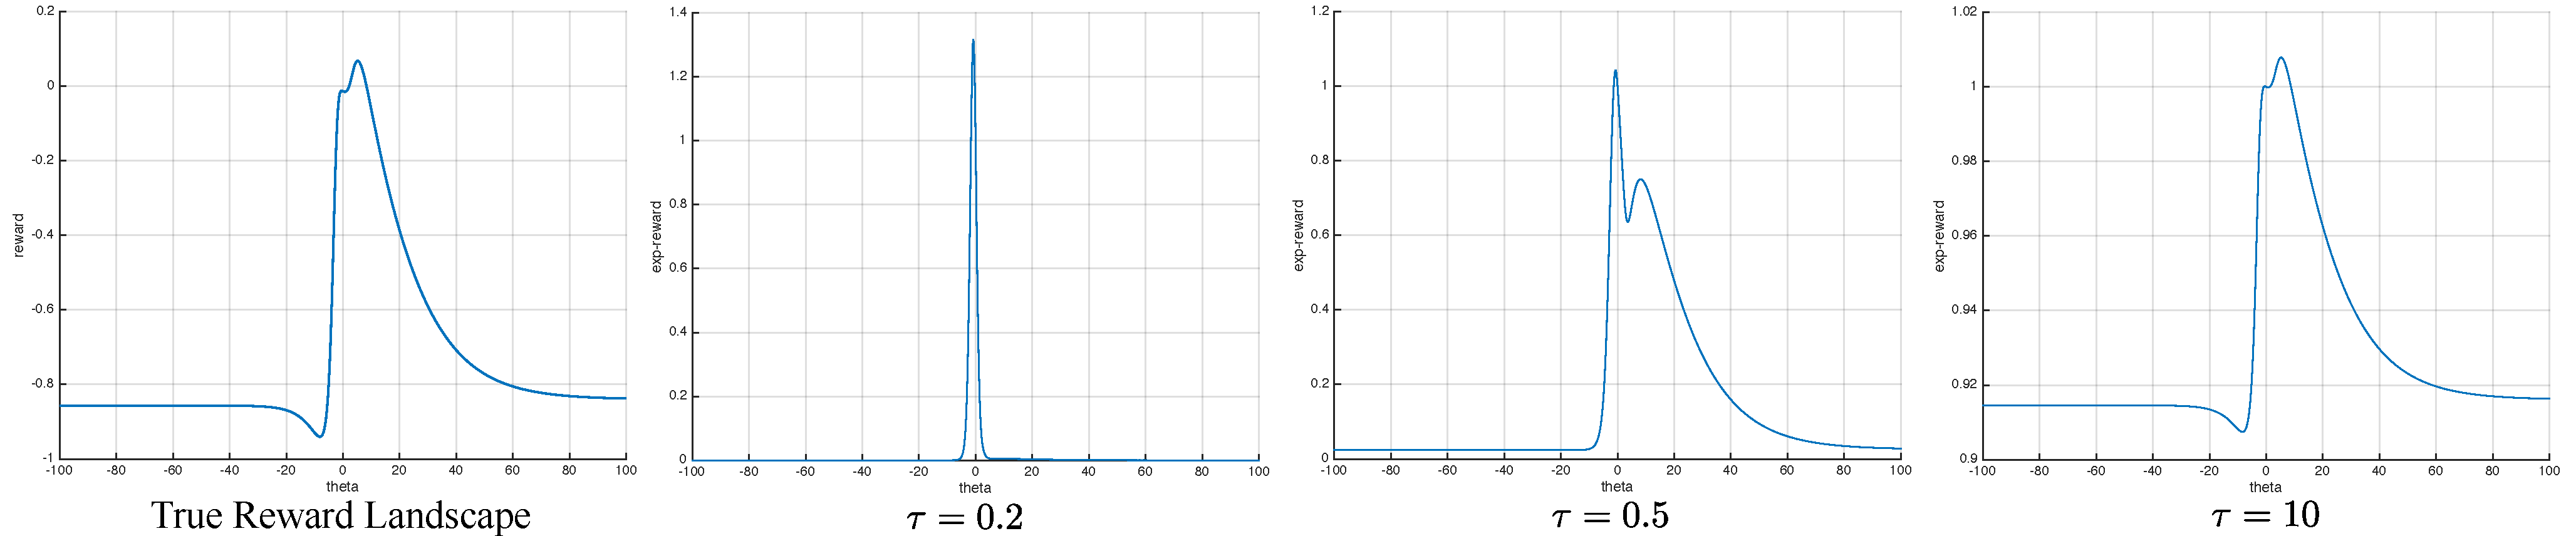
\includegraphics[width=1.0\linewidth]{./sr_simulation.pdf}
\end{center}
\caption{
Simulation result for true reward landscape and $\SR(\pi)$ with different value of $\tau$.} 
\label{fig:srsimulation}
\end{figure*}
 
\subsection{Learning }
\label{subsec:learning}
\todor[]{Maybe move this section to Appendix}
We now discuss the implementation details of REPMD. The full algorithm is presented in \cref{alg:repmd}.
Despite of its non-convexity, it can be verified that the lift step has an analytic solution
\begin{equation}
\label{eq:pitautauprime}
\bar{\pi}_{\tau,\tau^{\prime}}^*(\rho) \triangleq \frac{\refPi(\rho) \exp\left\{ \frac{r(\rho)-\tau^{\prime} \log \refPi(\rho) }{ \tau+\tau^{\prime}} \right\}}{ \sum_{\rho^{\prime}}{\refPi(\rho^{\prime}) \exp\left\{ \frac{r(\rho^{\prime})-\tau^{\prime} \log \refPi(\rho^{\prime})}{ \tau+\tau^{\prime}} \right\} } }.
\end{equation}
%First note that the \emph{unconstrained optimal policy} $\bar{\pi}_{\tau,\tau^{\prime}}^*$ in (\ref{eq:repmd}) has a closed form expression.
%To see that, note that $\argmin\nolimits_{\pi_\theta \in \Pi}\KL(\bar{\pi}_{\tau,\tau^{\prime}}^* \| \pi_\theta) = \argmin\nolimits_{\pi_\theta \in \Pi} \ep_{\rho \sim \bar{\pi}_{\tau,\tau^{\prime}}^* }  - \log \pi_\theta(\rho)$.
The project step in \cref{eq:repmd}, $\min\nolimits_{\pi_\theta \in \Pi}{\KL(\bm{ \bar{\pi}_{\tau,\tau^{\prime}}^* \| \pi_\theta }) }$, can be optimized via stochastic gradient descent, given that one can sample trajectories from $\bar{\pi}_{\tau,\tau^{\prime}}^*$ to estimate its gradient. To see this, note that $\argmin\nolimits_{\pi_\theta \in \Pi}\KL(\bar{\pi}_{\tau,\tau^{\prime}}^* \| \pi_\theta) = \argmin\nolimits_{\pi_\theta \in \Pi} \ep_{\rho \sim \bar{\pi}_{\tau,\tau^{\prime}}^* }  - \log \pi_\theta(\rho)$. The next theorem shows that sampling from $\bar{\pi}_{\tau,\tau^{\prime}}^*$ can be done using self-normalized importance sampling \citep{owen2013monte}, following the idea of UREX \citep{nachum2017improving}.
\begin{thm}
\label{thm:repmdgradientestimate}
Let $\omega_k = \frac{r(\rho_k) - \tau^{\prime} \log{\refPi(\rho_k)} }{\tau + \tau^{\prime}}$. Given $K$ \emph{i.i.d.} samples $\{\rho_1, \dots, \rho_K\}$ from the \emph{reference policy} $\refPi$, we have the following unbiased gradient estimator,
\begin{equation}
\label{eq:gradient_estimator}
	\nabla_{\theta} \KL(\bar{\pi}_{\tau,\tau^{\prime}}^* \| \pi_\theta)\approx -\sum\limits_{k=1}^K{ \frac{ \exp\left\{ \omega_k \right\} }{ \sum_{j=1}^K{ \exp\left\{ \omega_j \right\}}} \nabla_{\theta} \log{\pi_\theta(\rho_k)} },
\end{equation}
%	where 
%	\[
%	\omega_k = \frac{r(\rho_k) - \tau^{\prime} \log{\refPi(\rho_k)} }{\tau + \tau^{\prime}}.
%	\] 
\end{thm}














